% Who is doing what:
% Jordan - 2.4.1 question 1, max-flow
% Darrin - RB tree
% Logan  - 2.1.1, 2.2.1
% Kate   - Example of max-flow

\documentclass[12pt]{amsart}

\usepackage[margin=0.75in]{geometry}

% Image setup
\usepackage{graphicx}
\graphicspath{{./images/}}

\title{Exploration and Analysis of Red-Black Trees and Max Flow
    Algorithms}
\author{Jordan Dehmel, Kate Eckhart, Logan Humbert, Darrin Miller}
\date{Fall 2023}

\begin{document}

\maketitle

\tableofcontents

\section{Abstract}

    We explore various properties and real-world applications of
    red-black trees and max-flow optimization algorithms. We
    explore several algorithms for the later, and provide
    experimental comparative analysis of their performances.

\section{Introduction}

\section{Red-Black Trees}

\subsection{Theoretical Analysis}

    \textbf{Discuss the theoretical aspects of Red-Black Trees, including time and space
	complexity, best/worst/average-case scenarios, and any important properties.}
	
	Red-Black Trees are a special type of binary search tree that are self-balancing: they maintain their balance
    during insertions and deletions.
    
    Just as for any other type of binary search trees, for each node of a Red-Black Tree, all nodes in its left subtree have a value less than the node, and all nodes in its right subtree have a value greater than the node.
    
    Red-Black Trees have additional properties:
    
    \begin{itemize}
    	\item Each node of the tree is either colored red or black
    	\item The root and all leaves are black
    	\item Having two consecutive red nodes is not allowed on any path from the root to a leaf.
    	\item Every path from a node to any of its leaves contains the same number of black nodes.
    \end{itemize}
    
    Now, I will discuss the time complexity of Red-Black Trees.
    
    \begin{itemize}
    	\item For the search operation, it has a time complexity of O(1). It happens when the element being searched is found at the root of the tree.
    	It has an average and worst time complexity of O(log n), because the tree maintains balance, resulting in a logarithmic height.
    	
    	\item Concerning the insertion operation, it has a time complexity of O(1) in its best case, in which the new node is inserted at the root.
    	Its average and worst time complexities are O(log n). On average, the tree needs to be balanced, keeping the height logarithmic.
    	In the worst case, the tree needs restructuring, which takes logarithmic time.
    	
    	\item For the deletion operation, we have the exact same time complexities than for the insertion operation, for the same reasons.
    	
    	\item Finally, rotation operations are done in constant time.
    \end{itemize}
    
    Finally, I will expose the space complexity of Red-Black Trees.
    Each node in a Red-Black Tree requires constant space for the key, value, color information, and pointers to its children and parent. The overall space complexity is O(n), where n is the number of nodes in the tree.
    
    Moreover, during operations like insertion and deletion, some additional space may be required for temporary variables or recursive function calls.
    The auxiliary space complexity is O(log n) in the worst case, where log n is the height of the tree.
\subsection{Practical Implementation Details}

\subsection{Real-World Application}

\subsection{Theoretical Questions}

    \textbf{Prove that the height of a Red-Black tree with
    n nodes is guaranteed to be $O(log n)$ in the worst
    case scenario. Provide a rigorous mathematical proof.}
    
    In this proof, we will first prove that the height of a
    2-3-4 tree is limited by $O(log n)$. Then, we will prove
    that any valid red-black tree can be converted directly into
    a 2-3-4 tree. Finally, we will note that, so long as height
    is measured only in black links, tree height is maintained
    by this conversion.

    A 2-3-4 tree, by its nature, only grows by pushing the root
    "upwards". The only time at which the height of such a tree
    increases is when a 4-node at the root splits, sending a
    node upwards to become the new root. In this case, the
    height of the tree uniformly increases by one for all leaf
    nodes. This means that the height of the tree is precisely
    equal for all leaf nodes.

    Now we will examine the equivalency between red-black trees
    and 2-3-4 trees. We will show that each node in a 2-3-4 tree
    corresponds to exactly one black link in a red-black tree,
    and that the only additions needed are red links.

    First, we will consider a 2-node. This is a node with two
    output links. This is equivalent to the standard node in a
    binary tree- no modifications are needed to modify it into
    red-black tree form.

    Next, we will consider a 3-node. This is a node with three
    output links. The leftmost represents the subtree wherein
    all nodes are less than the lesser item in the node. The
    rightmost similarly represents the subtree wherein all nodes
    are larger than the greater item, and the middle represents
    the subtree containing nodes who fit neither of these trees.

\begin{center}
    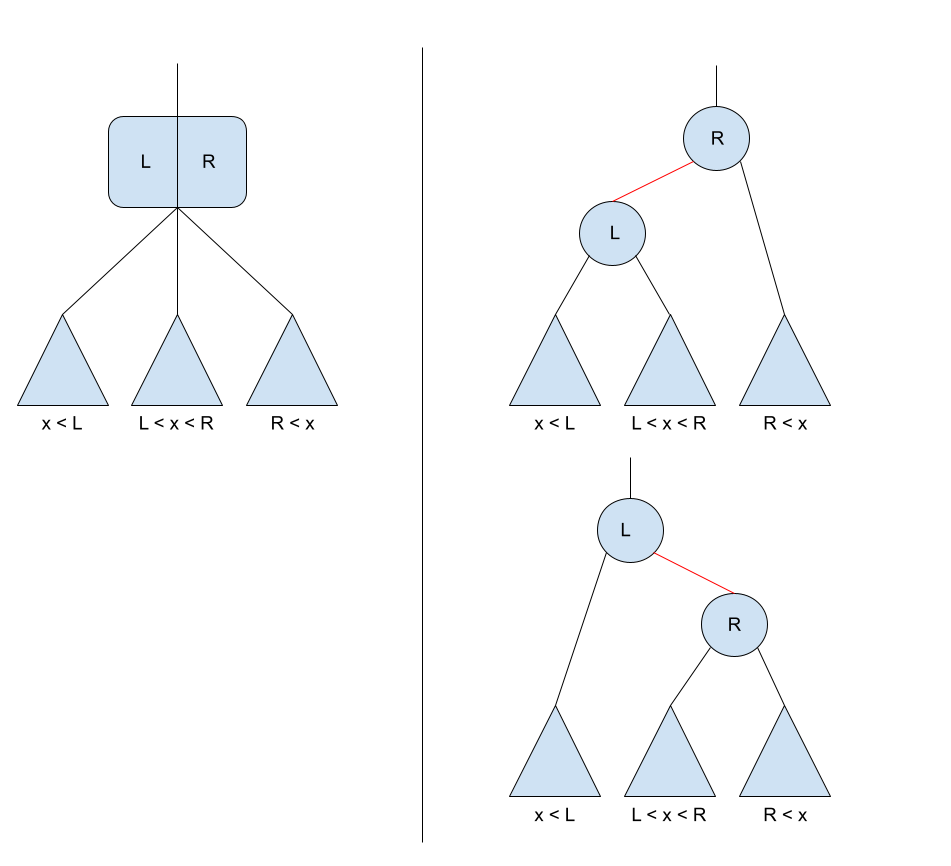
\includegraphics[width=0.65\textwidth]{rb_tree_1} \\
    A 3-node and its possible red-black tree versions. \\
    \vskip 1cm
\end{center}

    Since the height of a red-black tree is the number of black
    links the root must follow to get to a leaf, the two
    possible red-black subtrees above both have a height of $1$:
    the same height as the 2-3-4 tree they came from.

    The only remaining case is the 4-node. A 4-node usually only
    exists in a 2-3-4 tree for a moment before it is split
    apart. If we designate the $3$ items within the node as
    $a$, $b$, and $c$, then we say that (from left to right) the
    child links represent the ranges $x < a$, $a < x < b$,
    $b < x < c$, and $c < x$ for any item $x$ in the given
    child subtree. These cases, of course, can also be covered
    by an equivalent red-black tree, as shown below.

\begin{center}
    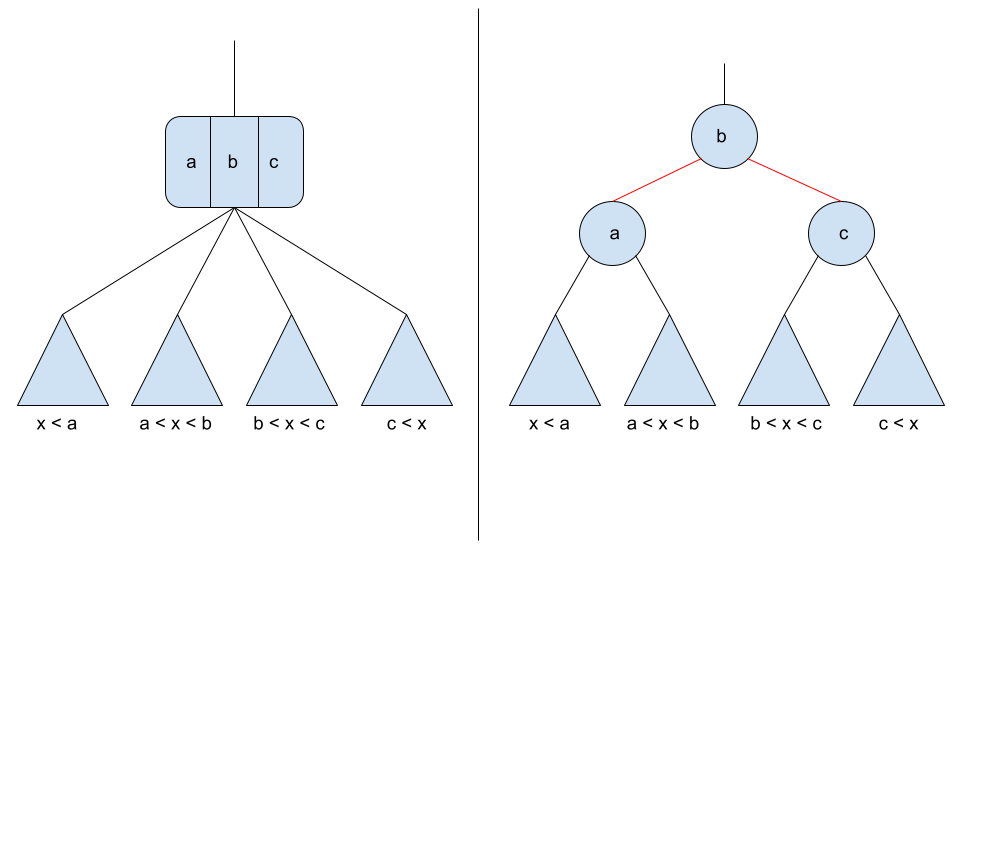
\includegraphics[width=0.65\textwidth]{rb_tree_2} \\
    A 4-node and its red-black tree version. \\
    \vskip 1cm
\end{center}

    Again, this red-black tree has the same height as its 2-3-4
    tree equivalent: $1$. Since we have accounted for all
    possible variations of red-black subtree herein, we can use
    the above rules to translate between red-black trees and
    2-3-4 trees. Therefore, any statement we make about 2-3-4
    trees holds for red-black trees.

    In the best-case scenario, a 2-3-4 tree (post 4-node
    splitting) containing $n$ nodes will have a height of
    $log_3(n)$, where every node is a 3-node. At worst case, it
    will have a height of $log_2(n)$, where every node is a
    2-node. Since red-black and 2-3-4 trees are equivalent, we
    can thusly say that the worst-case height of a red-black
    tree of size $n$ is limited by $log_2(n)$ black links.

    \newpage
    \textbf{Discuss how Red-Black trees are used in modern
    databases and file systems to maintain balanced structures.
    Explain the trade-offs and advantages of using Red-Black
    trees in these contexts.}

\section{Max Flow Algorithms}

\subsection{Theoretical Analysis}
    % Jordan

    We will begin by analyzing the time and space complexity
    of the \textbf{Ford-Fulkerson algorithm} for max flow, and
    use this to motivate the segue into the Edmonds-Karp
    algorithm.

    The Ford-Fulkerson algorithm works by repeatedly finding an
    augmenting path (a path which can traverse the graph from
    the source node to the sink node and contains some amount of
    unused capacity) and adding the minimal flow across this
    path to the flow of each edge within. When no such path can
    be found, the graph has reached its maximal flow, and an
    answer to the problem can be returned. The pseudocode for
    the Ford-Fulkerson algorithm is shown below.

\begin{verbatim}
// 1) Initialize
Set all edges in flow graph to zero
Set residual graph to input graph

// 2) Iterate
While an augmenting path exists:
    Get augmenting path
    Add augmenting path to flow graph
    Subtract augmenting path from residual graph
End while

// 3) Output
Set net flow to zero
For edge exiting source node:
    Increment net flow by edge flow
End for

Return net flow
\end{verbatim}

    The most ambiguous part of this process is
    \verb|get augmenting path|. This vagueness has lead some to
    classify this process the Ford-Fulkerson method, rather than
    algorithm, as the time complexity could be vastly changed by
    the specific implementation of this line. For clarity, we
    will continue to refer to it as an algorithm. In our
    implementation, we will simply interpret this line to mean
    "choose the first augmenting path"- more specifically, 
    "at each node, if multiple augmenting paths are present,
    choose the one leading to the lowest-indexed node from this
    point". That is to say, if the paths \verb|0 -> 1 -> 2| and
    \verb|0 -> 3 -> 2| both exists, our initial algorithm would
    choose the first.

    Using these definitions and the above pseudocode, we can
    begin algorithmic analyses of the algorithm. We will call
    the set of all vertices $\mathbb{V}$, and the number of
    vertices $\vert \mathbb{V} \vert$. Similarly, the set of all
    edges and the number thereof are $\mathbb{E}$ and
    $\vert \mathbb{E} \vert$, respectively.
    
    The algorithm starts by initializing its variables, marked
    section 1 in the above code. These operations take
    $\vert \mathbb{E} \vert$ each. Next, the algorithm iterates
    over the augmenting paths. For each iteration, it gets an
    augmenting path, adds the augmenting path to the flow, and
    subtracts it from the residual. This means that this section
    runs with time proportional to the number of augmenting
    paths times two times the length of the current path. Each
    pass of this iteration is guaranteed to add at least 1 unit
    to the net flow, so there will be at most $f^*$ iterations,
    where $f^*$ is the maximal flow. The final section of the
    algorithm (section 3, which computes the calculated net
    flow), runs in time proportional to the number of edges
    leading from the source node, which is at most
    $\vert \mathbb{E} \vert$.

    Tying everything together, we can say that the
    Ford-Fulkerson algorithm runs in time proportional to

\[
    2 \cdot \vert \mathbb{E} \vert + f^* \cdot \vert \mathbb{E} \vert + \vert \mathbb{E} \vert
\]

    Converting this to big-O notation, we find that the running
    time complexity of the Ford-Fulkerson algorithm as listed
    here is $O(f^* \vert \mathbb{E} \vert )$.

    As written here, the Ford-Fulkerson algorithm uses several
    auxiliary variables of equal size to the input graph.
    However, were the preservation of the input graph not
    necessary, the operations using these variables could easily
    be modified to work by modifying the input graph. This
    means that, under proper optimization, the Ford-Fulkerson
    algorithm runs with space complexity $O(1)$.

    Having now finished analyzing the Ford-Fulkerson algorithm,
    we can move on to the Edmonds-Karp algorithm. As proven
    above, the Ford-Fulkerson algorithm can only be proved to
    converge upon the solution in time proportional to the max
    flow value itself. Thus, it is particularly unsuited for
    graphs with large maximal flows. Additionally, the original
    specification for the Ford-Fulkerson algorithm left the
    specific method used to select the next augmenting path
    unspecified. The solution to both of these problems comes
    in the form of the \textbf{Edmonds-Karp algorithm}.

    The Edmonds-Karp algorithm is a specific implementation of
    the Ford-Fulkerson method / algorithm wherein the next
    augmenting path to be chosen is the shortest one. This
    shortest path is chosen via breadth-first-search of the
    network. This allows the time complexity of the algorithm
    to become independent from $f*$.

    The pseudocode for the Edmonds-Karp algorithm is listed
    below.

\begin{verbatim}
// 1) Initialize
Set all edges in flow graph to zero
Set residual graph to input graph

// 2) Iterate
While an augmenting path exists:
    Get shortest augmenting path via BFS
    Add augmenting path to flow graph
    Subtract augmenting path from residual graph
End while

// 3) Output
Set net flow to zero
For edge exiting source node:
    Increment net flow by edge flow
End for

Return net flow
\end{verbatim}

\subsection{Practical Implementation Details}
    % Jordan

\begin{center}
    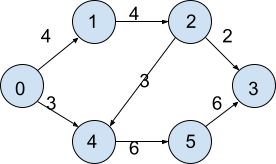
\includegraphics[width=0.65\textwidth]{graph} \\
    A benchmark graph for max-flow. \\
    \vskip 1cm
\end{center}

\subsection{Real-World Application}

\subsection{Theoretical Questions}

    \textbf{Describe the concept of augmenting paths and
    their role in the Ford-Fulkerson algorithm. Prove that the
    algorithm terminates and converges to the maximum flow in
    finite time, even for non-integer capacities.}

    \textbf{Explain the Min-Cut Max-Flow Theorem and its
    significance in the context of network flows. How can this
    theorem be used to find a maximum flow and minimum cut in a
    flow network?}

\section{Real-World Problem Solving}

\section{Comparative Analysis and Reporting}

\subsection{Red-Black Trees}

\subsection{Max Flow Algorithms}
    % Jordan

    Below is a graph of running times from a series of
    experimental runs of the Ford-Fulkerson (FF) and
    Edmonds-Karp (EK) algorithms on various randomly-generated
    graphs.

\begin{center}
    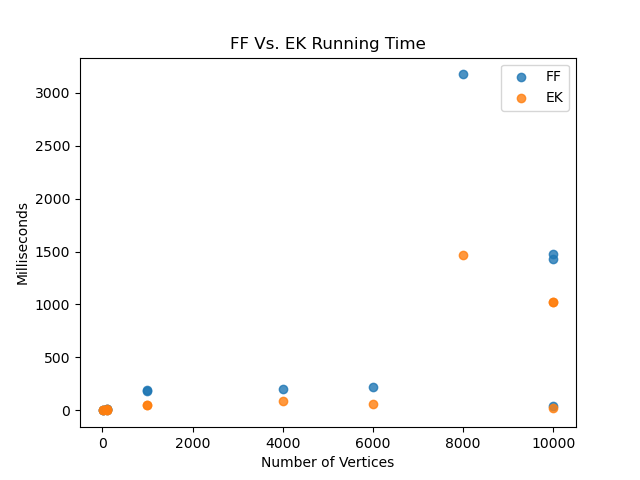
\includegraphics[width=0.65\textwidth]{mf_algorithm_comparison} \\
    The Ford-Fulkerson (FF) algorithm vs the Edmonds-Karp (EK)
    algorithm on randomly generated graphs of various size. \\
    \vskip 1cm
\end{center}

    Clearly, the Edmonds-Karp algorithm performs reliably
    better than the original Ford-Fulkerson one, especially for
    large graphs.

    The below graph shows the number of augmenting paths present
    in graphs of various sizes.

\begin{center}
    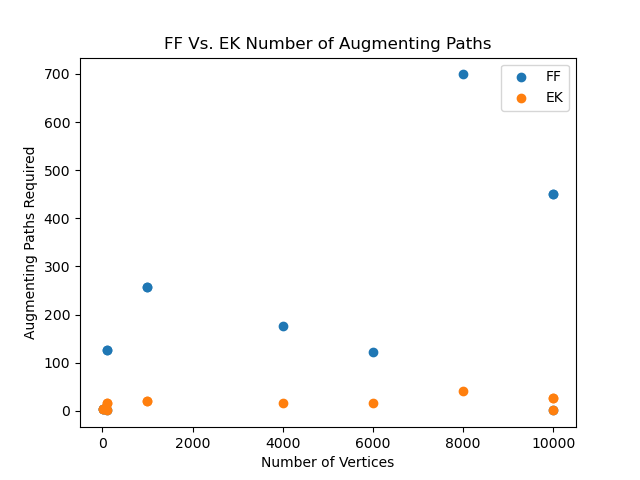
\includegraphics[width=0.65\textwidth]{mf_passes_comparison.png} \\
    The Ford-Fulkerson (FF) algorithm vs the Edmonds-Karp (EK)
    algorithm on various graphs, by number of passes required. \\
    \vskip 1cm
\end{center}

\section{Conclusion}

\section{References}

\begin{itemize}
    \item https://sedgewick.io/wp-content/themes/sedgewick/papers/2008LLRB.pdf
    \item https://www.cs.purdue.edu/homes/ayg/CS251/slides/chap13b.pdf
    \item https://www.geeksforgeeks.org/ford-fulkerson-algorithm-for-maximum-flow-problem/
    \item https://brilliant.org/wiki/ford-fulkerson-algorithm/    
    \item https://brilliant.org/wiki/edmonds-karp-algorithm/
\end{itemize}

\end{document}